\documentclass{article}
% pre\'ambulo

\usepackage{lmodern}
\usepackage[T1]{fontenc}
\usepackage[spanish,activeacute]{babel}
\usepackage{mathtools}
\usepackage{graphicx}
\usepackage{listings}
\usepackage{tabu}
\usepackage{hyperref}
\usepackage[utf8]{inputenc}
\usepackage{multicol}
\usepackage{amsmath}
\usepackage{amssymb}
\usepackage{enumerate}
\usepackage{amsthm}
\usepackage{wrapfig}
\usepackage{esvect}
\usepackage{subcaption}
%\usepackage{wasysym}
\usepackage{mathabx}

\spanishdecimal{.}




% Default fixed font does not support bold face
\DeclareFixedFont{\ttb}{T1}{txtt}{bx}{n}{8} % for bold
\DeclareFixedFont{\ttm}{T1}{txtt}{m}{n}{8}  % for normal

% Custom colors
\usepackage[usenames,dvipsnames]{color}
\definecolor{deepblue}{rgb}{0,0,0.5}
\definecolor{deepred}{rgb}{0.6,0,0}
\definecolor{deepgreen}{rgb}{0,0.5,0}

% Python style for highlighting
\newcommand\pythonstyle{\lstset{
language=Python,
basicstyle=\ttm,
otherkeywords={self},             % Add keywords here
keywordstyle=\ttb\color{deepblue},
emph={MyClass,__init__},          % Custom highlighting
emphstyle=\ttb\color{deepred},    % Custom highlighting style
stringstyle=\color{deepgreen},
frame=tb,                         % Any extra options here
showstringspaces=false            % 
}}


% Python environment
\lstnewenvironment{python}[1][]
{
\pythonstyle
\lstset{#1}
}
{}

% Python for external files
\newcommand\pythonexternal[2][]{{
\pythonstyle
\lstinputlisting[#1]{#2}}}

% Python for inline
\newcommand\pythoninline[1]{{\pythonstyle\lstinline!#1!}}

\usepackage{amsmath} % or simply amstext
\newcommand{\angstrom}{\text{\normalfont\AA}}
\newcommand*{\everymodeprime}{\ensuremath{\prime}}

\title{Tarea 1}
\author{Francisco Felipe Carrasco Varela}

\usepackage{vmargin}

\setpapersize{A4}
\setmargins{1.82cm}       % margen izquierdo
{1.3cm}                        % margen superior
{17.5cm}                      % anchura del texto
{23.42cm}                    % altura del texto
{10pt}                           % altura de los encabezados
{1cm}                           % espacio entre el texto y los encabezados
{0pt}                             % altura del pie de página
{2cm}                           % espacio entre el texto y el pie de página

\usepackage{array,booktabs,tabularx,caption, ragged2e}
\newcolumntype{C}{>{\centering\arraybackslash}X}

\begin{document}
\begin{minipage}{2.3cm}

\includegraphics[width=2cm]{../logo_byn.png}
\vspace{0.5cm}
\end{minipage}
\begin{minipage}{\linewidth}
\textsc{\raggedright \footnotesize
Pontificia Universidad Católica de Chile \\
Facultad de Física -- Instituto de Astrof'isica \\
Astronom'ia -- AST0111 \\
Primer Semestre 2020}
\end{minipage}
\begin{center}
{\LARGE \textbf{Ayudant'ia 8}}

\vspace{3mm}

Profesora: Viviana Guzm'an

Ayudantes: Camila Aravena Gonz'alez (\texttt{cfaravena1$@$uc.cl}) -- Francisco Carrasco Varela (\texttt{ffcarrasco$@$uc.cl})

\end{center}
\begin{center}
\noindent\rule{12cm}{0.4pt}
\end{center}

\textbf{Problema 1. Conceptos generales}

\vspace{3mm}

\begin{enumerate}[a)] 


\item ¿C'omo se pueden clasificar las estrellas seg'un su espectro? ?`Qu'e nos puede decir este espectro?
\item Si observo una estrella cuya magnitud aparente en filtro $V$ es $m_V = -4$ y otra estrella cuya magnitud es $m_V = 2$. ?`Cu'al es m'as brillante y por qu'e? ?`C'omo se comparan sus luminosidades asumiendo que ambas estrellas tuviesen el mismo radio?
\item En astronom'ia generalmente se define el color como la resta de la magnitud medida para un mismo objeto en dos filtros distintos. Por ejemplo: medimos la magnitud de una estrella en filtro ``$B$'' 'esta nos da una magnitud de $m_B = 3.8$ y al medir la magnitud en filtro ``$V$'' 'esta nos da $m_V = 4.0$. Por convenci'on, siempre se resta el filtro m'as rojo al filtro m'as azul; por ejemplo, en este caso, tendr'iamos $B-V = -0.02$. ?`Qu'e se puede inferir entonces de una estrella si medimos su magnitud en 2 filtros distintos?
\item ¿Qu'e es un diagrama Hertzprung-Russel, tambi'en conocido como diagrama H-R o diagrama Color-Magnitud, y por qu'e es tan utilizado en astronom'ia?
\end{enumerate}

\textbf{Problema 2. Estrellas de baja masa vs. estrellas de alta masa}

\vspace{3mm}


\begin{enumerate}[a)]
\item ?`Cu'ales son los rangos (aproximados\footnote{Digo ``aproximados'' porque en la literatura siempre encontrar'a valores \emph{similares}, pero \emph{no necesariamente iguales}. No hay una definici'on 'unica.}) para las estrellas de baja, intermedia y alta masa?

\item De los rangos anteriores en base a la masa, ?`cu'ales esperar'ia que fuesen las estrellas que m'as o menos viven y por qu'e?


\item ?`Se espera que una estrella de alta masa sea m'as o menos luminosa que una estrella como el Sol? ?`Y qu'e es lo que se espera para el tiempo de vida de una estrella masiva con respecto a una estrella no masiva? Compare sus respuestas de la luminosidad y tiempo de vida que se espera para una estrella de $1 \ M_\odot$ con otra de $10 \ M_\odot$. ?`Qu'e puede inferir de estos resultados? Dato (quiz'as) 'util: Asuma que la luminosidad del Sol es $L \sim 4 \times 10^{26} \ \text{W}$ y su tiempo de vida es $\tau_\odot \approx 10^{10} \ \text{yr}$.

\item Hasta donde sabemos, el Sol est'a constantemente fusionando hidr'ogeno en su n'ucleo cuando 'este se encuentra en la fase de Secuencia principal (o en ingl'es, Main-Sequence [MS]). Sin embargo, el proceso a trav'es del cual el hidr'ogeno es ``quemado'' dentro del n'ucleo de las estrellas es distinto. 

Para estrellas en MS, ?`en qu'e se diferencia la quema de hidr'ogeno para una estrella de baja masa con una de alta masa?

%\item Las estrellas circumpolares son estrellas que nunca se ponen bajo el horizonte para el observador local; o estrellas que nunca son visibles sobre el horizonte (nunca salen). 

%\begin{enumerate}[i)]
%\item Calcule el rango de declinaciones para estos dos grupos de estrellas (que se ven y no se ven) para un observador a una latitud L.

%\item ?`A qu'e latitud(es) en la Tierra el Sol nunca se podr'a cuando sea el solsticio de verano (en el hemisferio norte)?

%\item Basado en los dos sub-problemas anteriores, ?`existe alguna latitud en la Tierra donde el Sol nunca se pondr'a cuando sea el equinnocio vernal? De ser as'i, ?`d'onde?
%\end{enumerate}

\begin{figure}
\centering
  \begin{subfigure}{6cm}
    \centering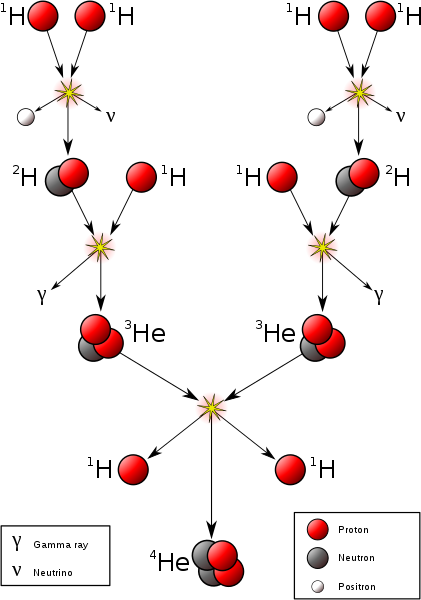
\includegraphics[width=6cm]{p-p.png}
    \caption{Cadena prot'on-prot'on}
  \end{subfigure}
  \begin{subfigure}{6cm}
    \centering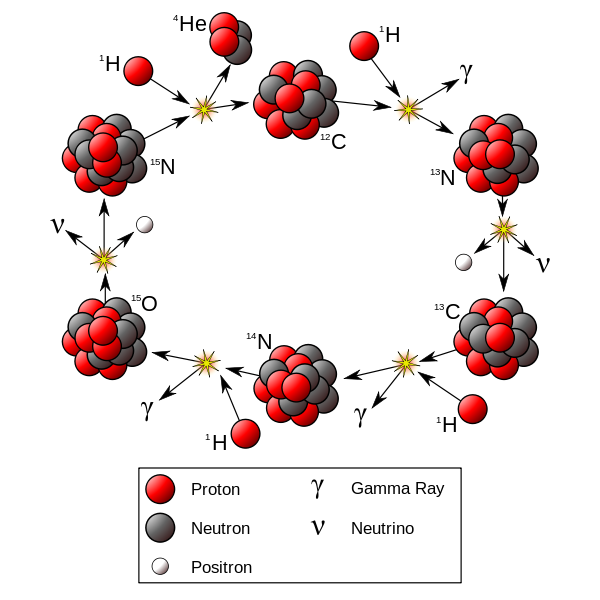
\includegraphics[width=8.5cm]{cno.png}
    \caption{Ciclo CNO}
  \end{subfigure}
  \caption{Distintas reacciones de fusi'on que se pueden generar dentro de una estrella. Cu'al es la que va a dominar depende de la masa de la estrella.}
\end{figure} 
\vspace{3mm}


\end{enumerate}

\newpage

\textbf{Problema 3. El Sol}

\vspace{3mm}


Considere una estrella como el Sol, con una masa de aproximadamente $M_\odot \approx 2 \times 10^{30} \ \text{kg}$ y una luminosidad de aproximadamente $L \sim 4 \times 10^{26} \ \text{W}$, con $\text{W} = \text{kg} \ \text{m}^2/\text{s}^3$. Por simplicidad, asuma que el Sol estaba
compuesto por hidrógeno y nada m'as al momento de su formaci'on. Considere que el Sol emite energ'ia
transformando núcleos de hidrógeno (con masa dada por $m_{\rm H} = 1.67 \times 10^{-27} \ \text{kg}$) en núcleos de helio ($m_{\rm He} = 6.65 \times 10^{-27} \ \text{kg}$).

\begin{enumerate} [a)]
\item ?`Cu'antos 'atomos de hidr'ogeno se necesitan para crear un 'atomo de helio?
\item ?`Cu'al es, aproximadamente, la diferencia porcentual de masa entre los ingredientes y los productos de la reacci'on nuclear para el Sol? ?`Es la diferencia positiva o negativa? ?`Qu'e implica aquello?
\item Si todo el hidr'ogeno del Sol se transforma en Helio, ?`c'omo cambia su masa?
\item ?`Cu'anta energ'ia producir'ia ese proceso? Por simplicidad, recuerde una famosa ecuaci'on del mism'isimo Albert Einstein y asuma $c^2 = 10^{17} \ \text{m}^2\cdot \text{s}^{-2}$.
\item Si el Sol mantiene su luminosidad constante, ?`por cu'anto tiempo puede durar as'i (que todo el hidr'ogeno se transforme en helio)?
\item ?`C'omo se compara el resultado con ``la vida 'util real'' del Sol, que es unos $\tau_\odot \approx 10^{10} \ \text{yr}$? ?`Puede decir algo de la similitud (o discrepancia) del resultado que ha hallado?
\end{enumerate}


\end{document}